Sebelum mengetahui teknologi apa saja yang digunakan serta tata cara pembuatan sistem voice cloning ini, akan lebih baik apabila kita memahami terlebih dahulu mengenai sistem \textit{Text to Speech (TTS)}.

\section{Text to Speech (TTS)}
Text to Speech merupakan proses pembuatan suara melalui inputan berupa text. mungkin teman-teman bingung, bagaimana bisa text berubah menjadi suara, sementara text itu hanya dapat kita lihat menggunakan panca indra kita yaitu mata sedangkan suara merupakan sesuatu yang tidak bisa kita lihat menggunakan mata tetapi bisa kita dengar menggunakan telingga. Text to Speech ini ada untuk menjawab kebingungan teman-teman tersebut. Di zaman sekarang ini, dimana teknologi sudah semakin canggih, mengubah teks menjadi suara bukanlah hal yang sulit untuk dilakukan, apalagi setelah teman-teman mengenal deep learning, machine learning, dan artificial intelligence. Bagi teman-teman yang masih belum kenal, yuk kenalan dulu.
\begin{figure}[H]
        \centerline{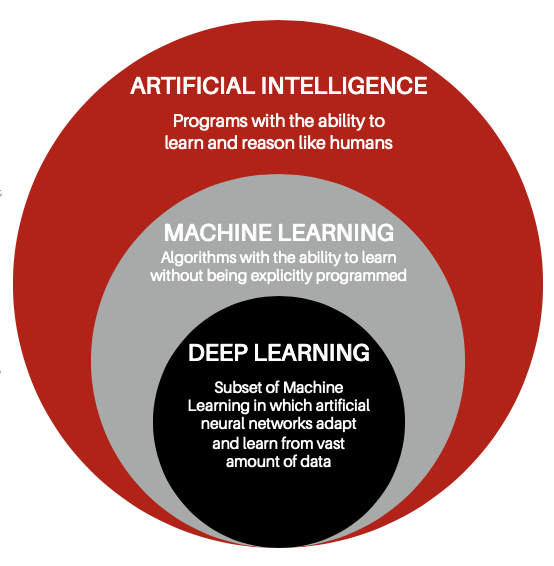
\includegraphics[scale=.75]{figures/korelasi}}
        \caption{Korelasi antara Deep Learning, Machine Learning, dan Artificial Intelligence}
		\label{korelasi}
\end{figure}

\subsection{Artificial Intelligence}
Artificial Intelligence (AI) merupakan kecerdasan yang dibuat dan diberikan atau diterapkan pada program komputer yang diharapkan memiliki kecerdasan seperti manusia sehingga memiliki kemampuan memahami, merencanakan, mengambil keputusan, dan problem solving. Dalam pembuatannya, setiap algoritma memungkinkan mesin untuk meniru, mengembangkan, dan berprilaku seperti manusia. Sederhananya AI itu merupakan sebuah teknologi yang memungkinkan kita menciptakan sebuah mesin yang memiliki kecerdasan berdasarkan pada perintah atau algoritma yang kita berikan pada program tersebut. Algoritma berupa langkah-langkah yang kita lakukan dalam menyelesaikan suatu permasalahan. Misalnya kita ingin menciptakan mesin yang dapat menjawab semua pertanyaan kita seperti chatbot, maka kita membutuhkan algoritma atau langkah-langkah apa yang dilakukan oleh chatbot untuk memahami dan mampu memberikan respon secara cepat dan tepat kepada kita.

Artificial Intelligence dibuat dengan 3 tujuan, diantaranya:
\begin{enumerate}
\item Tujuan utama, Membuat mesin menjadi lebih pintar dan terus mengalami peningkatan seiring dengan perkembangan teknologi.
\item Tujuan ilmiah, Memahami apa itu kecerdasan buatan sehingga dapat dimanfaatkan untuk membuat mesin yang lebih cerdas dalam membantu dan memecahkan masalah secara efektif dan efisien.
\item Tujuan entrepreneurial, Membuat mesin lebih bermanfaat sehingga memudahkan manusia dalam melakukan perkerjaan dan memecahkan masalah secara cepat, tepat, dan lebih teliti.
\end{enumerate}

\subsection{Machine Learning}
Machine Learning (ML) merupakan bagian dari Artificial Intelligence yang ditambahkan dengan metode-metode statistika dengan tujuan agar mesin dapat meningkat-kan pengalamannya berdasarkan kepada data-data yang ada dan dilatih pada mesin tersebut. Dengan begitu mesin dapat melakukan tugas tertentu berdasarkan data dan algoritma yang diterapkan padanya. Data dan algoritma yang dirancang membuat mesin terus mengalami peningkatan dari waktu ke waktu. Sebagai contoh, pada pembuatan sistem untuk memprediksi tweet yang bersifat positif, negatif, atau netral kita akan membutuhkan data tweet dari para pengguna twitter, kita bisa dapatkan melalui API yang telah disediakan oleh twitter. Pada tahap pertama, kita mengambil 100 data tweet yang terdiri dari tweet positif, negatif, dan netral. Lalu kita melatih mesin menggunakan 100 data tersebut dan menggunakan algoritma naive bayes untuk mengetahui apakah data hasil prediksi kita sama dengan data tweet aslinya dan menghitung akurasi dari algoritma yang telah kita buat. Pada tahap pertama akurasi menunjukkan angkat 90\% dan ketika kita melakukan training kembali kepada algoritma atau model yang telah kita buat dengan menggunakan data yang lebih banyak lagi maka mesin akan menjadi lebih terlatih dan kemungkinan kesalahan prediksi menjadi sangat kecil bahkan akurasi yang didapatkan dari model bisa mencapai 99\% atau bahkan kita bisa mengganti algoritma yang kita gunakan menggunakan algoritma lainnya yang menghasilkan akurasi yang lebih baik dari model atau algoritma kita sebelumnya. Hal inilah yang dimaksud dengan machine learning, ada data dan algoritma serta perhitungan-perhitungan yang sering kita jumpai dalam statistika seperti perhitungan akurasi, rata-rata (mean), median, recall, precision, dll.

\subsection{Deep Learning}
Setelah mengenal AI dan ML saatnya kita mengenal Deep Learning (DL) yang merupakan bagian dari Machine Learning yang berkaitan dengan algoritma yang berdasarkan pada struktur dan fungsi otak atau sering dikenal sebagai jaringan saraf tiruan. Pada dasarnya Deep Learning memiliki konsep seperti Machine Learning hanya saja dalam konteks yang lebih dalam. Contohnya, pada deep learning kita ingin membuat mesin dapat mengetahui apakah hewan yang ada digambar merupakan seekor anjing atau kucing, maka kita akan membuat algoritma untuk melakukan pengecekan seperti melakukan pengecekan pada bentuk ekor, bentuk telinga, apakah memiliki kumis atau tidak, dan ciri-ciri lainnya yang membuat kucing dan anjing terlihat berbeda tanpa kita perlu memberikan fitur pembedanya atau fitur mana yang lebih penting untuk dapat mengidentifikasi hewan tersebut secara manual. Deep Learning dapat mengetahui fitur tersebut tanpa kita beritahu secara manual seperti pada Machine Learning seperti terlihat pada gambar \ref{deep learning}. Oleh karena itu Deep Learning dianggap sebagai otak utama yang menciptakan kecerdasan buatan yang lebih manusiawi.
\begin{figure}[H]
        \centerline{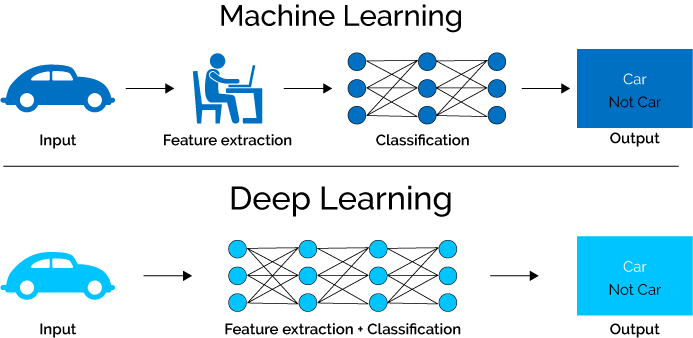
\includegraphics[scale=.45]{figures/deeplearning}}
        \caption{Perbedaan Machine Learning dan Deep Learning}
		\label{deep learning}
\end{figure}

Text to Speech termasuk bagian dari Deep Learning lebih tepatnya Neural Network. Neural Network merupakan cabang ilmu yang mengadopsi cara berpikir dan cara bekerja otak manusia yang memberikan rangsangan/stimulus (input), melalukan proses, dan menghasilkan sesuatu (output). Output dihasilkan dari inputan yang diberikan dan proses yang dilakukan oleh otak manusia. Kemampuan otak untuk memproses inputan atau informasi ini yang akan membuat otak manusia selalu mempelajari hal-hal baru dan terus berkembang, begitupun dengan mesin yang diberikan kecerdasan buatan atau AI. Contohnya saja ketika kita berusia 5 tahun dan otak kita belum memahami informasi-informasi yang sulit seperti pelajaran matematika dasar, menambah dan mengurangi ataupun membagi dan mengalikan angka. Setelah kita mempelajarinya selama 6 tahun di Sekolah Dasar maka otak kita sekarang bisa memahaminya bahkan hal tersebut merupakan hal yang sangat gampang. Pada dasarnya konsep AI sama dengan otak manusia yang selalu berkembang dan mempelajari hal-hal yang baru berdasarkan inputan atau informasi apa yang diberikan kepada otak dan otak akan memproses inputan tersebut hingga dapat memahami dan mengeluarkan hasil dari proses tersebut (output).
Dalam pembuatan voice cloning ini kita akan mengajarkan kepada mesin cara membaca text dan mengucapkannya dengan menggunakan suara seperti yang kita contohkan, oleh karena itu kita membutuhkan sistem text to speech.


\section{Cara Kerja TTS}
Cara kerja TTS terdiri dari 2 proses, dapat dilihat pada gambar \ref{cara kerja}:
\begin{enumerate}
\item Model Teks ke Spektogram, model ini mengubah teks menjadi fitur yang selaras dengan waktu seperti spektogram, mel-spektogram, atau frekuensi F0 dan fitur linguistik lainnya. Ada beberapa model yang bisa digunakan untuk mengubah teks menjadi spektogram, diantaranya yaitu Tacotron, Tacotron2, Deep Voice 3, dll. Model ini juga disebut sebagai model encoder-decoder.
\item Model spektogram ke audio, model ini akan mengonversi spektogram yang dihasilkan menjadi audio. Model ini disebut sebagai vocoder. Beberapa model yang banyak digunakan untuk membuat vocoder yaitu WaveGlow, Griffin-Lim Algorithm, WaveNet, dll.
Model Tacotron-2 sebagai model encoder-decoder dan model WaveNet yang dimodifikasi sebagai vocoder akan dibahas secara mendalam pada buku ini.
\end{enumerate}
\begin{figure}[H]
        \centerline{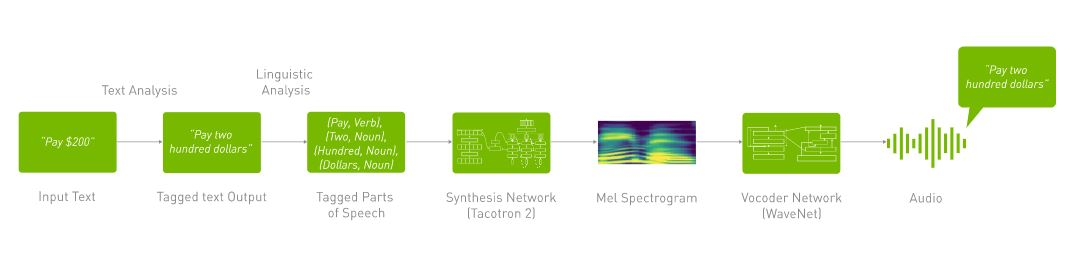
\includegraphics[scale=.40]{figures/cara_kerja_tts}}
        \caption{Cara Kerja Text to Speech (TTS)}
		\label{cara kerja}
\end{figure}
